% !TeX spellcheck = en_GB
\documentclass[a4paper]{article}
% ****************************************************************************************************
% classicthesis-config.tex
% formerly known as loadpackages.sty, classicthesis-ldpkg.sty, and classicthesis-preamble.sty
% Use it at the beginning of your ClassicThesis.tex, or as a LaTeX Preamble
% in your ClassicThesis.{tex,lyx} with % ****************************************************************************************************
% classicthesis-config.tex
% formerly known as loadpackages.sty, classicthesis-ldpkg.sty, and classicthesis-preamble.sty
% Use it at the beginning of your ClassicThesis.tex, or as a LaTeX Preamble
% in your ClassicThesis.{tex,lyx} with % ****************************************************************************************************
% classicthesis-config.tex
% formerly known as loadpackages.sty, classicthesis-ldpkg.sty, and classicthesis-preamble.sty
% Use it at the beginning of your ClassicThesis.tex, or as a LaTeX Preamble
% in your ClassicThesis.{tex,lyx} with \input{classicthesis-config}
% ****************************************************************************************************
% If you like the classicthesis, then I would appreciate a postcard.
% My address can be found in the file ClassicThesis.pdf. A collection
% of the postcards I received so far is available online at
% http://postcards.miede.de
% ****************************************************************************************************


% ****************************************************************************************************
% 0. Set the encoding of your files. UTF-8 is the only sensible encoding nowadays. If you can't read
% äöüßáéçèê∂åëæƒÏ€ then change the encoding setting in your editor, not the line below. If your editor
% does not support utf8 use another editor!
% ****************************************************************************************************
\PassOptionsToPackage{utf8}{inputenc}
  \usepackage{inputenc}

\PassOptionsToPackage{T1}{fontenc} % T2A for cyrillics
  \usepackage{fontenc}


% ****************************************************************************************************
% 1. Configure classicthesis for your needs here, e.g., remove "drafting" below
% in order to deactivate the time-stamp on the pages
% (see ClassicThesis.pdf for more information):
% ****************************************************************************************************
\PassOptionsToPackage{
  drafting=true,    % print version information on the bottom of the pages
  tocaligned=false, % the left column of the toc will be aligned (no indentation)
  dottedtoc=false,  % page numbers in ToC flushed right
  eulerchapternumbers=true, % use AMS Euler for chapter font (otherwise Palatino)
  linedheaders=false,       % chaper headers will have line above and beneath
  floatperchapter=true,     % numbering per chapter for all floats (i.e., Figure 1.1)
  eulermath=true,  % use awesome Euler fonts for mathematical formulae (only with pdfLaTeX)
  beramono=true,    % toggle a nice monospaced font (w/ bold)
  palatino=true,    % deactivate standard font for loading another one, see the last section at the end of this file for suggestions
  style=classicthesis % classicthesis, arsclassica
}{classicthesis}


% ****************************************************************************************************
% 2. Personal data and user ad-hoc commands (insert your own data here)
% ****************************************************************************************************
\newcommand{\myTitle}{A Multi-Node Quantum Network with Defects in Diamond\xspace}
\newcommand{\mySubtitle}{Ph.D. proposal\xspace}
%\newcommand{\myDegree}{Doktor-Ingenieur (Dr.-Ing.)\xspace}
\newcommand{\myName}{Matteo Pompili\xspace}
%\newcommand{\myProf}{Put name here\xspace}
%\newcommand{\myOtherProf}{Put name here\xspace}
\newcommand{\mySupervisor}{Ronald Hanson\xspace}
%\newcommand{\myFaculty}{Put data here\xspace}
%\newcommand{\myDepartment}{Put data here\xspace}
%\newcommand{\myUni}{Put data here\xspace}
%\newcommand{\myLocation}{Saarbrücken\xspace}
\newcommand{\myTime}{November 23, 2018\xspace}
\newcommand{\myVersion}{\classicthesis}

% ********************************************************************
% Setup, finetuning, and useful commands
% ********************************************************************
\providecommand{\mLyX}{L\kern-.1667em\lower.25em\hbox{Y}\kern-.125emX\@}
\newcommand{\ie}{i.\,e.}
\newcommand{\Ie}{I.\,e.}
\newcommand{\eg}{e.\,g.}
\newcommand{\Eg}{E.\,g.}
% ****************************************************************************************************


% ****************************************************************************************************
% 3. Loading some handy packages
% ****************************************************************************************************
% ********************************************************************
% Packages with options that might require adjustments
% ********************************************************************
\PassOptionsToPackage{british, UKenglish}{babel} % change this to your language(s), main language last
% Spanish languages need extra options in order to work with this template
%\PassOptionsToPackage{spanish,es-lcroman}{babel}
    \usepackage{babel}

\usepackage{csquotes}
\PassOptionsToPackage{%
  backend=biber,bibencoding=utf8, %instead of bibtex
%  backend=bibtex8,bibencoding=ascii,%
  language=auto,%
  style=numeric-comp,%
  %style=authoryear-comp, % Author 1999, 2010
  %bibstyle=authoryear,dashed=false, % dashed: substitute rep. author with ---
  sorting=none, % name, year, title
  maxbibnames=10, % default: 3, et al.
  %backref=true,%
  natbib=true % natbib compatibility mode (\citep and \citet still work)
}{biblatex}
    \usepackage{biblatex}

\PassOptionsToPackage{fleqn}{amsmath}       % math environments and more by the AMS
  \usepackage{amsmath}

% ********************************************************************
% General useful packages
% ********************************************************************
\usepackage{graphicx} %
\usepackage{scrhack} % fix warnings when using KOMA with listings package
\usepackage{xspace} % to get the spacing after macros right
\PassOptionsToPackage{printonlyused,smaller}{acronym}
  \usepackage{acronym} % nice macros for handling all acronyms in the thesis
  %\renewcommand{\bflabel}[1]{{#1}\hfill} % fix the list of acronyms --> no longer working
  %\renewcommand*{\acsfont}[1]{\textsc{#1}}
  %\renewcommand*{\aclabelfont}[1]{\acsfont{#1}}
  %\def\bflabel#1{{#1\hfill}}
  \def\bflabel#1{{\acsfont{#1}\hfill}}
  \def\aclabelfont#1{\acsfont{#1}}
% ****************************************************************************************************
%\usepackage{pgfplots} % External TikZ/PGF support (thanks to Andreas Nautsch)
%\usetikzlibrary{external}
%\tikzexternalize[mode=list and make, prefix=ext-tikz/]
% ****************************************************************************************************


% ****************************************************************************************************
% 4. Setup floats: tables, (sub)figures, and captions
% ****************************************************************************************************
\usepackage{tabularx} % better tables
  \setlength{\extrarowheight}{3pt} % increase table row height
\newcommand{\tableheadline}[1]{\multicolumn{1}{l}{\spacedlowsmallcaps{#1}}}
\newcommand{\myfloatalign}{\centering} % to be used with each float for alignment
\usepackage{subfig}
% ****************************************************************************************************


% ****************************************************************************************************
% 5. Setup code listings
% ****************************************************************************************************
\usepackage{listings}
%\lstset{emph={trueIndex,root},emphstyle=\color{BlueViolet}}%\underbar} % for special keywords
\lstset{language=[LaTeX]Tex,%C++,
  morekeywords={PassOptionsToPackage,selectlanguage},
  keywordstyle=\color{RoyalBlue},%\bfseries,
  basicstyle=\small\ttfamily,
  %identifierstyle=\color{NavyBlue},
  commentstyle=\color{Green}\ttfamily,
  stringstyle=\rmfamily,
  numbers=none,%left,%
  numberstyle=\scriptsize,%\tiny
  stepnumber=5,
  numbersep=8pt,
  showstringspaces=false,
  breaklines=true,
  %frameround=ftff,
  %frame=single,
  belowcaptionskip=.75\baselineskip
  %frame=L
}
% ****************************************************************************************************




% ****************************************************************************************************
% 6. Last calls before the bar closes
% ****************************************************************************************************
% ********************************************************************
% Her Majesty herself
% ********************************************************************
\usepackage{classicthesis}


% ********************************************************************
% Fine-tune hyperreferences (hyperref should be called last)
% ********************************************************************
\hypersetup{%
  %draft, % hyperref's draft mode, for printing see below
  %  colorlinks=true, linktocpage=true, pdfstartpage=3, pdfstartview=FitV,%
  % uncomment the following line if you want to have black links (e.g., for printing)
  colorlinks=false, linktocpage=false, pdfstartpage=3, pdfstartview=FitV, pdfborder={0 0 0},%
  breaklinks=true, pageanchor=true,%
  pdfpagemode=UseNone, %
  % pdfpagemode=UseOutlines,%
  plainpages=false, bookmarksnumbered, bookmarksopen=true, bookmarksopenlevel=1,%
  hypertexnames=true, pdfhighlight=/O,%nesting=true,%frenchlinks,%
  urlcolor=CTurl, linkcolor=CTlink, citecolor=CTcitation, %pagecolor=RoyalBlue,%
  %urlcolor=Black, linkcolor=Black, citecolor=Black, %pagecolor=Black,%
  pdftitle={\myTitle},%
  pdfauthor={\textcopyright\ \myName},%
  pdfsubject={},%
  pdfkeywords={},%
  pdfcreator={pdfLaTeX},%
  pdfproducer={LaTeX with hyperref and classicthesis}%
}


% ********************************************************************
% Setup autoreferences (hyperref and babel)
% ********************************************************************
% There are some issues regarding autorefnames
% http://www.tex.ac.uk/cgi-bin/texfaq2html?label=latexwords
% you have to redefine the macros for the
% language you use, e.g., american, ngerman
% (as chosen when loading babel/AtBeginDocument)
% ********************************************************************
\makeatletter
\@ifpackageloaded{babel}%
  {%
    \addto\extrasamerican{%
      \renewcommand*{\figureautorefname}{Figure}%
      \renewcommand*{\tableautorefname}{Table}%
      \renewcommand*{\partautorefname}{Part}%
      \renewcommand*{\chapterautorefname}{Chapter}%
      \renewcommand*{\sectionautorefname}{Section}%
      \renewcommand*{\subsectionautorefname}{Section}%
      \renewcommand*{\subsubsectionautorefname}{Section}%
    }%
    \addto\extrasngerman{%
      \renewcommand*{\paragraphautorefname}{Absatz}%
      \renewcommand*{\subparagraphautorefname}{Unterabsatz}%
      \renewcommand*{\footnoteautorefname}{Fu\"snote}%
      \renewcommand*{\FancyVerbLineautorefname}{Zeile}%
      \renewcommand*{\theoremautorefname}{Theorem}%
      \renewcommand*{\appendixautorefname}{Anhang}%
      \renewcommand*{\equationautorefname}{Gleichung}%
      \renewcommand*{\itemautorefname}{Punkt}%
    }%
      % Fix to getting autorefs for subfigures right (thanks to Belinda Vogt for changing the definition)
      \providecommand{\subfigureautorefname}{\figureautorefname}%
    }{\relax}
\makeatother


% ********************************************************************
% Development Stuff
% ********************************************************************
\listfiles
%\PassOptionsToPackage{l2tabu,orthodox,abort}{nag}
%  \usepackage{nag}
%\PassOptionsToPackage{warning, all}{onlyamsmath}
%  \usepackage{onlyamsmath}


% ****************************************************************************************************
% 7. Further adjustments (experimental)
% ****************************************************************************************************
% ********************************************************************
% Changing the text area
% ********************************************************************
%\areaset[current]{312pt}{761pt} % 686 (factor 2.2) + 33 head + 42 head \the\footskip
%\setlength{\marginparwidth}{7em}%
%\setlength{\marginparsep}{2em}%

% ********************************************************************
% Using different fonts
% ********************************************************************
%\usepackage[oldstylenums]{kpfonts} % oldstyle notextcomp
% \usepackage[osf]{libertine}
%\usepackage[light,condensed,math]{iwona}
%\renewcommand{\sfdefault}{iwona}
%\usepackage{lmodern} % <-- no osf support :-(
%\usepackage{cfr-lm} %
%\usepackage[urw-garamond]{mathdesign} <-- no osf support :-(
%\usepackage[default,osfigures]{opensans} % scale=0.95
%\usepackage[sfdefault]{FiraSans}
% \usepackage[opticals,mathlf]{MinionPro} % onlytext
% ********************************************************************
%\usepackage[largesc,osf]{newpxtext}
%\linespread{1.05} % a bit more for Palatino
% Used to fix these:
% https://bitbucket.org/amiede/classicthesis/issues/139/italics-in-pallatino-capitals-chapter
% https://bitbucket.org/amiede/classicthesis/issues/45/problema-testatine-su-classicthesis-style
% ********************************************************************
% ****************************************************************************************************

% ****************************************************************************************************
% If you like the classicthesis, then I would appreciate a postcard.
% My address can be found in the file ClassicThesis.pdf. A collection
% of the postcards I received so far is available online at
% http://postcards.miede.de
% ****************************************************************************************************


% ****************************************************************************************************
% 0. Set the encoding of your files. UTF-8 is the only sensible encoding nowadays. If you can't read
% äöüßáéçèê∂åëæƒÏ€ then change the encoding setting in your editor, not the line below. If your editor
% does not support utf8 use another editor!
% ****************************************************************************************************
\PassOptionsToPackage{utf8}{inputenc}
  \usepackage{inputenc}

\PassOptionsToPackage{T1}{fontenc} % T2A for cyrillics
  \usepackage{fontenc}


% ****************************************************************************************************
% 1. Configure classicthesis for your needs here, e.g., remove "drafting" below
% in order to deactivate the time-stamp on the pages
% (see ClassicThesis.pdf for more information):
% ****************************************************************************************************
\PassOptionsToPackage{
  drafting=true,    % print version information on the bottom of the pages
  tocaligned=false, % the left column of the toc will be aligned (no indentation)
  dottedtoc=false,  % page numbers in ToC flushed right
  eulerchapternumbers=true, % use AMS Euler for chapter font (otherwise Palatino)
  linedheaders=false,       % chaper headers will have line above and beneath
  floatperchapter=true,     % numbering per chapter for all floats (i.e., Figure 1.1)
  eulermath=true,  % use awesome Euler fonts for mathematical formulae (only with pdfLaTeX)
  beramono=true,    % toggle a nice monospaced font (w/ bold)
  palatino=true,    % deactivate standard font for loading another one, see the last section at the end of this file for suggestions
  style=classicthesis % classicthesis, arsclassica
}{classicthesis}


% ****************************************************************************************************
% 2. Personal data and user ad-hoc commands (insert your own data here)
% ****************************************************************************************************
\newcommand{\myTitle}{A Multi-Node Quantum Network with Defects in Diamond\xspace}
\newcommand{\mySubtitle}{Ph.D. proposal\xspace}
%\newcommand{\myDegree}{Doktor-Ingenieur (Dr.-Ing.)\xspace}
\newcommand{\myName}{Matteo Pompili\xspace}
%\newcommand{\myProf}{Put name here\xspace}
%\newcommand{\myOtherProf}{Put name here\xspace}
\newcommand{\mySupervisor}{Ronald Hanson\xspace}
%\newcommand{\myFaculty}{Put data here\xspace}
%\newcommand{\myDepartment}{Put data here\xspace}
%\newcommand{\myUni}{Put data here\xspace}
%\newcommand{\myLocation}{Saarbrücken\xspace}
\newcommand{\myTime}{November 23, 2018\xspace}
\newcommand{\myVersion}{\classicthesis}

% ********************************************************************
% Setup, finetuning, and useful commands
% ********************************************************************
\providecommand{\mLyX}{L\kern-.1667em\lower.25em\hbox{Y}\kern-.125emX\@}
\newcommand{\ie}{i.\,e.}
\newcommand{\Ie}{I.\,e.}
\newcommand{\eg}{e.\,g.}
\newcommand{\Eg}{E.\,g.}
% ****************************************************************************************************


% ****************************************************************************************************
% 3. Loading some handy packages
% ****************************************************************************************************
% ********************************************************************
% Packages with options that might require adjustments
% ********************************************************************
\PassOptionsToPackage{british, UKenglish}{babel} % change this to your language(s), main language last
% Spanish languages need extra options in order to work with this template
%\PassOptionsToPackage{spanish,es-lcroman}{babel}
    \usepackage{babel}

\usepackage{csquotes}
\PassOptionsToPackage{%
  backend=biber,bibencoding=utf8, %instead of bibtex
%  backend=bibtex8,bibencoding=ascii,%
  language=auto,%
  style=numeric-comp,%
  %style=authoryear-comp, % Author 1999, 2010
  %bibstyle=authoryear,dashed=false, % dashed: substitute rep. author with ---
  sorting=none, % name, year, title
  maxbibnames=10, % default: 3, et al.
  %backref=true,%
  natbib=true % natbib compatibility mode (\citep and \citet still work)
}{biblatex}
    \usepackage{biblatex}

\PassOptionsToPackage{fleqn}{amsmath}       % math environments and more by the AMS
  \usepackage{amsmath}

% ********************************************************************
% General useful packages
% ********************************************************************
\usepackage{graphicx} %
\usepackage{scrhack} % fix warnings when using KOMA with listings package
\usepackage{xspace} % to get the spacing after macros right
\PassOptionsToPackage{printonlyused,smaller}{acronym}
  \usepackage{acronym} % nice macros for handling all acronyms in the thesis
  %\renewcommand{\bflabel}[1]{{#1}\hfill} % fix the list of acronyms --> no longer working
  %\renewcommand*{\acsfont}[1]{\textsc{#1}}
  %\renewcommand*{\aclabelfont}[1]{\acsfont{#1}}
  %\def\bflabel#1{{#1\hfill}}
  \def\bflabel#1{{\acsfont{#1}\hfill}}
  \def\aclabelfont#1{\acsfont{#1}}
% ****************************************************************************************************
%\usepackage{pgfplots} % External TikZ/PGF support (thanks to Andreas Nautsch)
%\usetikzlibrary{external}
%\tikzexternalize[mode=list and make, prefix=ext-tikz/]
% ****************************************************************************************************


% ****************************************************************************************************
% 4. Setup floats: tables, (sub)figures, and captions
% ****************************************************************************************************
\usepackage{tabularx} % better tables
  \setlength{\extrarowheight}{3pt} % increase table row height
\newcommand{\tableheadline}[1]{\multicolumn{1}{l}{\spacedlowsmallcaps{#1}}}
\newcommand{\myfloatalign}{\centering} % to be used with each float for alignment
\usepackage{subfig}
% ****************************************************************************************************


% ****************************************************************************************************
% 5. Setup code listings
% ****************************************************************************************************
\usepackage{listings}
%\lstset{emph={trueIndex,root},emphstyle=\color{BlueViolet}}%\underbar} % for special keywords
\lstset{language=[LaTeX]Tex,%C++,
  morekeywords={PassOptionsToPackage,selectlanguage},
  keywordstyle=\color{RoyalBlue},%\bfseries,
  basicstyle=\small\ttfamily,
  %identifierstyle=\color{NavyBlue},
  commentstyle=\color{Green}\ttfamily,
  stringstyle=\rmfamily,
  numbers=none,%left,%
  numberstyle=\scriptsize,%\tiny
  stepnumber=5,
  numbersep=8pt,
  showstringspaces=false,
  breaklines=true,
  %frameround=ftff,
  %frame=single,
  belowcaptionskip=.75\baselineskip
  %frame=L
}
% ****************************************************************************************************




% ****************************************************************************************************
% 6. Last calls before the bar closes
% ****************************************************************************************************
% ********************************************************************
% Her Majesty herself
% ********************************************************************
\usepackage{classicthesis}


% ********************************************************************
% Fine-tune hyperreferences (hyperref should be called last)
% ********************************************************************
\hypersetup{%
  %draft, % hyperref's draft mode, for printing see below
  %  colorlinks=true, linktocpage=true, pdfstartpage=3, pdfstartview=FitV,%
  % uncomment the following line if you want to have black links (e.g., for printing)
  colorlinks=false, linktocpage=false, pdfstartpage=3, pdfstartview=FitV, pdfborder={0 0 0},%
  breaklinks=true, pageanchor=true,%
  pdfpagemode=UseNone, %
  % pdfpagemode=UseOutlines,%
  plainpages=false, bookmarksnumbered, bookmarksopen=true, bookmarksopenlevel=1,%
  hypertexnames=true, pdfhighlight=/O,%nesting=true,%frenchlinks,%
  urlcolor=CTurl, linkcolor=CTlink, citecolor=CTcitation, %pagecolor=RoyalBlue,%
  %urlcolor=Black, linkcolor=Black, citecolor=Black, %pagecolor=Black,%
  pdftitle={\myTitle},%
  pdfauthor={\textcopyright\ \myName},%
  pdfsubject={},%
  pdfkeywords={},%
  pdfcreator={pdfLaTeX},%
  pdfproducer={LaTeX with hyperref and classicthesis}%
}


% ********************************************************************
% Setup autoreferences (hyperref and babel)
% ********************************************************************
% There are some issues regarding autorefnames
% http://www.tex.ac.uk/cgi-bin/texfaq2html?label=latexwords
% you have to redefine the macros for the
% language you use, e.g., american, ngerman
% (as chosen when loading babel/AtBeginDocument)
% ********************************************************************
\makeatletter
\@ifpackageloaded{babel}%
  {%
    \addto\extrasamerican{%
      \renewcommand*{\figureautorefname}{Figure}%
      \renewcommand*{\tableautorefname}{Table}%
      \renewcommand*{\partautorefname}{Part}%
      \renewcommand*{\chapterautorefname}{Chapter}%
      \renewcommand*{\sectionautorefname}{Section}%
      \renewcommand*{\subsectionautorefname}{Section}%
      \renewcommand*{\subsubsectionautorefname}{Section}%
    }%
    \addto\extrasngerman{%
      \renewcommand*{\paragraphautorefname}{Absatz}%
      \renewcommand*{\subparagraphautorefname}{Unterabsatz}%
      \renewcommand*{\footnoteautorefname}{Fu\"snote}%
      \renewcommand*{\FancyVerbLineautorefname}{Zeile}%
      \renewcommand*{\theoremautorefname}{Theorem}%
      \renewcommand*{\appendixautorefname}{Anhang}%
      \renewcommand*{\equationautorefname}{Gleichung}%
      \renewcommand*{\itemautorefname}{Punkt}%
    }%
      % Fix to getting autorefs for subfigures right (thanks to Belinda Vogt for changing the definition)
      \providecommand{\subfigureautorefname}{\figureautorefname}%
    }{\relax}
\makeatother


% ********************************************************************
% Development Stuff
% ********************************************************************
\listfiles
%\PassOptionsToPackage{l2tabu,orthodox,abort}{nag}
%  \usepackage{nag}
%\PassOptionsToPackage{warning, all}{onlyamsmath}
%  \usepackage{onlyamsmath}


% ****************************************************************************************************
% 7. Further adjustments (experimental)
% ****************************************************************************************************
% ********************************************************************
% Changing the text area
% ********************************************************************
%\areaset[current]{312pt}{761pt} % 686 (factor 2.2) + 33 head + 42 head \the\footskip
%\setlength{\marginparwidth}{7em}%
%\setlength{\marginparsep}{2em}%

% ********************************************************************
% Using different fonts
% ********************************************************************
%\usepackage[oldstylenums]{kpfonts} % oldstyle notextcomp
% \usepackage[osf]{libertine}
%\usepackage[light,condensed,math]{iwona}
%\renewcommand{\sfdefault}{iwona}
%\usepackage{lmodern} % <-- no osf support :-(
%\usepackage{cfr-lm} %
%\usepackage[urw-garamond]{mathdesign} <-- no osf support :-(
%\usepackage[default,osfigures]{opensans} % scale=0.95
%\usepackage[sfdefault]{FiraSans}
% \usepackage[opticals,mathlf]{MinionPro} % onlytext
% ********************************************************************
%\usepackage[largesc,osf]{newpxtext}
%\linespread{1.05} % a bit more for Palatino
% Used to fix these:
% https://bitbucket.org/amiede/classicthesis/issues/139/italics-in-pallatino-capitals-chapter
% https://bitbucket.org/amiede/classicthesis/issues/45/problema-testatine-su-classicthesis-style
% ********************************************************************
% ****************************************************************************************************

% ****************************************************************************************************
% If you like the classicthesis, then I would appreciate a postcard.
% My address can be found in the file ClassicThesis.pdf. A collection
% of the postcards I received so far is available online at
% http://postcards.miede.de
% ****************************************************************************************************


% ****************************************************************************************************
% 0. Set the encoding of your files. UTF-8 is the only sensible encoding nowadays. If you can't read
% äöüßáéçèê∂åëæƒÏ€ then change the encoding setting in your editor, not the line below. If your editor
% does not support utf8 use another editor!
% ****************************************************************************************************
\PassOptionsToPackage{utf8}{inputenc}
  \usepackage{inputenc}

\PassOptionsToPackage{T1}{fontenc} % T2A for cyrillics
  \usepackage{fontenc}


% ****************************************************************************************************
% 1. Configure classicthesis for your needs here, e.g., remove "drafting" below
% in order to deactivate the time-stamp on the pages
% (see ClassicThesis.pdf for more information):
% ****************************************************************************************************
\PassOptionsToPackage{
  drafting=true,    % print version information on the bottom of the pages
  tocaligned=false, % the left column of the toc will be aligned (no indentation)
  dottedtoc=false,  % page numbers in ToC flushed right
  eulerchapternumbers=true, % use AMS Euler for chapter font (otherwise Palatino)
  linedheaders=false,       % chaper headers will have line above and beneath
  floatperchapter=true,     % numbering per chapter for all floats (i.e., Figure 1.1)
  eulermath=true,  % use awesome Euler fonts for mathematical formulae (only with pdfLaTeX)
  beramono=true,    % toggle a nice monospaced font (w/ bold)
  palatino=true,    % deactivate standard font for loading another one, see the last section at the end of this file for suggestions
  style=classicthesis % classicthesis, arsclassica
}{classicthesis}


% ****************************************************************************************************
% 2. Personal data and user ad-hoc commands (insert your own data here)
% ****************************************************************************************************
\newcommand{\myTitle}{A Multi-Node Quantum Network with Defects in Diamond\xspace}
\newcommand{\mySubtitle}{Ph.D. proposal\xspace}
%\newcommand{\myDegree}{Doktor-Ingenieur (Dr.-Ing.)\xspace}
\newcommand{\myName}{Matteo Pompili\xspace}
%\newcommand{\myProf}{Put name here\xspace}
%\newcommand{\myOtherProf}{Put name here\xspace}
\newcommand{\mySupervisor}{Ronald Hanson\xspace}
%\newcommand{\myFaculty}{Put data here\xspace}
%\newcommand{\myDepartment}{Put data here\xspace}
%\newcommand{\myUni}{Put data here\xspace}
%\newcommand{\myLocation}{Saarbrücken\xspace}
\newcommand{\myTime}{November 23, 2018\xspace}
\newcommand{\myVersion}{\classicthesis}

% ********************************************************************
% Setup, finetuning, and useful commands
% ********************************************************************
\providecommand{\mLyX}{L\kern-.1667em\lower.25em\hbox{Y}\kern-.125emX\@}
\newcommand{\ie}{i.\,e.}
\newcommand{\Ie}{I.\,e.}
\newcommand{\eg}{e.\,g.}
\newcommand{\Eg}{E.\,g.}
% ****************************************************************************************************


% ****************************************************************************************************
% 3. Loading some handy packages
% ****************************************************************************************************
% ********************************************************************
% Packages with options that might require adjustments
% ********************************************************************
\PassOptionsToPackage{british, UKenglish}{babel} % change this to your language(s), main language last
% Spanish languages need extra options in order to work with this template
%\PassOptionsToPackage{spanish,es-lcroman}{babel}
    \usepackage{babel}

\usepackage{csquotes}
\PassOptionsToPackage{%
  backend=biber,bibencoding=utf8, %instead of bibtex
%  backend=bibtex8,bibencoding=ascii,%
  language=auto,%
  style=numeric-comp,%
  %style=authoryear-comp, % Author 1999, 2010
  %bibstyle=authoryear,dashed=false, % dashed: substitute rep. author with ---
  sorting=none, % name, year, title
  maxbibnames=10, % default: 3, et al.
  %backref=true,%
  natbib=true % natbib compatibility mode (\citep and \citet still work)
}{biblatex}
    \usepackage{biblatex}

\PassOptionsToPackage{fleqn}{amsmath}       % math environments and more by the AMS
  \usepackage{amsmath}

% ********************************************************************
% General useful packages
% ********************************************************************
\usepackage{graphicx} %
\usepackage{scrhack} % fix warnings when using KOMA with listings package
\usepackage{xspace} % to get the spacing after macros right
\PassOptionsToPackage{printonlyused,smaller}{acronym}
  \usepackage{acronym} % nice macros for handling all acronyms in the thesis
  %\renewcommand{\bflabel}[1]{{#1}\hfill} % fix the list of acronyms --> no longer working
  %\renewcommand*{\acsfont}[1]{\textsc{#1}}
  %\renewcommand*{\aclabelfont}[1]{\acsfont{#1}}
  %\def\bflabel#1{{#1\hfill}}
  \def\bflabel#1{{\acsfont{#1}\hfill}}
  \def\aclabelfont#1{\acsfont{#1}}
% ****************************************************************************************************
%\usepackage{pgfplots} % External TikZ/PGF support (thanks to Andreas Nautsch)
%\usetikzlibrary{external}
%\tikzexternalize[mode=list and make, prefix=ext-tikz/]
% ****************************************************************************************************


% ****************************************************************************************************
% 4. Setup floats: tables, (sub)figures, and captions
% ****************************************************************************************************
\usepackage{tabularx} % better tables
  \setlength{\extrarowheight}{3pt} % increase table row height
\newcommand{\tableheadline}[1]{\multicolumn{1}{l}{\spacedlowsmallcaps{#1}}}
\newcommand{\myfloatalign}{\centering} % to be used with each float for alignment
\usepackage{subfig}
% ****************************************************************************************************


% ****************************************************************************************************
% 5. Setup code listings
% ****************************************************************************************************
\usepackage{listings}
%\lstset{emph={trueIndex,root},emphstyle=\color{BlueViolet}}%\underbar} % for special keywords
\lstset{language=[LaTeX]Tex,%C++,
  morekeywords={PassOptionsToPackage,selectlanguage},
  keywordstyle=\color{RoyalBlue},%\bfseries,
  basicstyle=\small\ttfamily,
  %identifierstyle=\color{NavyBlue},
  commentstyle=\color{Green}\ttfamily,
  stringstyle=\rmfamily,
  numbers=none,%left,%
  numberstyle=\scriptsize,%\tiny
  stepnumber=5,
  numbersep=8pt,
  showstringspaces=false,
  breaklines=true,
  %frameround=ftff,
  %frame=single,
  belowcaptionskip=.75\baselineskip
  %frame=L
}
% ****************************************************************************************************




% ****************************************************************************************************
% 6. Last calls before the bar closes
% ****************************************************************************************************
% ********************************************************************
% Her Majesty herself
% ********************************************************************
\usepackage{classicthesis}


% ********************************************************************
% Fine-tune hyperreferences (hyperref should be called last)
% ********************************************************************
\hypersetup{%
  %draft, % hyperref's draft mode, for printing see below
  %  colorlinks=true, linktocpage=true, pdfstartpage=3, pdfstartview=FitV,%
  % uncomment the following line if you want to have black links (e.g., for printing)
  colorlinks=false, linktocpage=false, pdfstartpage=3, pdfstartview=FitV, pdfborder={0 0 0},%
  breaklinks=true, pageanchor=true,%
  pdfpagemode=UseNone, %
  % pdfpagemode=UseOutlines,%
  plainpages=false, bookmarksnumbered, bookmarksopen=true, bookmarksopenlevel=1,%
  hypertexnames=true, pdfhighlight=/O,%nesting=true,%frenchlinks,%
  urlcolor=CTurl, linkcolor=CTlink, citecolor=CTcitation, %pagecolor=RoyalBlue,%
  %urlcolor=Black, linkcolor=Black, citecolor=Black, %pagecolor=Black,%
  pdftitle={\myTitle},%
  pdfauthor={\textcopyright\ \myName},%
  pdfsubject={},%
  pdfkeywords={},%
  pdfcreator={pdfLaTeX},%
  pdfproducer={LaTeX with hyperref and classicthesis}%
}


% ********************************************************************
% Setup autoreferences (hyperref and babel)
% ********************************************************************
% There are some issues regarding autorefnames
% http://www.tex.ac.uk/cgi-bin/texfaq2html?label=latexwords
% you have to redefine the macros for the
% language you use, e.g., american, ngerman
% (as chosen when loading babel/AtBeginDocument)
% ********************************************************************
\makeatletter
\@ifpackageloaded{babel}%
  {%
    \addto\extrasamerican{%
      \renewcommand*{\figureautorefname}{Figure}%
      \renewcommand*{\tableautorefname}{Table}%
      \renewcommand*{\partautorefname}{Part}%
      \renewcommand*{\chapterautorefname}{Chapter}%
      \renewcommand*{\sectionautorefname}{Section}%
      \renewcommand*{\subsectionautorefname}{Section}%
      \renewcommand*{\subsubsectionautorefname}{Section}%
    }%
    \addto\extrasngerman{%
      \renewcommand*{\paragraphautorefname}{Absatz}%
      \renewcommand*{\subparagraphautorefname}{Unterabsatz}%
      \renewcommand*{\footnoteautorefname}{Fu\"snote}%
      \renewcommand*{\FancyVerbLineautorefname}{Zeile}%
      \renewcommand*{\theoremautorefname}{Theorem}%
      \renewcommand*{\appendixautorefname}{Anhang}%
      \renewcommand*{\equationautorefname}{Gleichung}%
      \renewcommand*{\itemautorefname}{Punkt}%
    }%
      % Fix to getting autorefs for subfigures right (thanks to Belinda Vogt for changing the definition)
      \providecommand{\subfigureautorefname}{\figureautorefname}%
    }{\relax}
\makeatother


% ********************************************************************
% Development Stuff
% ********************************************************************
\listfiles
%\PassOptionsToPackage{l2tabu,orthodox,abort}{nag}
%  \usepackage{nag}
%\PassOptionsToPackage{warning, all}{onlyamsmath}
%  \usepackage{onlyamsmath}


% ****************************************************************************************************
% 7. Further adjustments (experimental)
% ****************************************************************************************************
% ********************************************************************
% Changing the text area
% ********************************************************************
%\areaset[current]{312pt}{761pt} % 686 (factor 2.2) + 33 head + 42 head \the\footskip
%\setlength{\marginparwidth}{7em}%
%\setlength{\marginparsep}{2em}%

% ********************************************************************
% Using different fonts
% ********************************************************************
%\usepackage[oldstylenums]{kpfonts} % oldstyle notextcomp
% \usepackage[osf]{libertine}
%\usepackage[light,condensed,math]{iwona}
%\renewcommand{\sfdefault}{iwona}
%\usepackage{lmodern} % <-- no osf support :-(
%\usepackage{cfr-lm} %
%\usepackage[urw-garamond]{mathdesign} <-- no osf support :-(
%\usepackage[default,osfigures]{opensans} % scale=0.95
%\usepackage[sfdefault]{FiraSans}
% \usepackage[opticals,mathlf]{MinionPro} % onlytext
% ********************************************************************
%\usepackage[largesc,osf]{newpxtext}
%\linespread{1.05} % a bit more for Palatino
% Used to fix these:
% https://bitbucket.org/amiede/classicthesis/issues/139/italics-in-pallatino-capitals-chapter
% https://bitbucket.org/amiede/classicthesis/issues/45/problema-testatine-su-classicthesis-style
% ********************************************************************
% ****************************************************************************************************

\usepackage{geometry}
\geometry{lmargin=2cm,rmargin=2cm,bmargin=2cm,tmargin=2cm}
% ACRONYMS
\usepackage[printonlyused]{acronym}
\acrodef{NV}{Nitrogen-Vacancy}
\acrodef{ESR}{Early Stage Researcher}
\acrodef{ITN}{Innovative Training Network}
\acrodef{MSCA}{Marie Skłodowska-Curie Actions}
\acrodef{SCE}{Single Click Entanglement}
\acrodef{MW}{microwave}
\acrodef{BS}{beam-splitter}
\acrodef{SLOCC}{stochastic local operations and classical communication}
\acrodef{GHZ}{Greenberger-Horne-Zeilinger}
\acrodef{AWG}{Arbitrary Waveform Generator}
\acrodef{QKD}{Quantum Key Distribution}
\acrodef{RF}{Radio Frequency}
\acrodef{BQC}{Blind Quantum Computation}
\acrodef{DD}{Dynamical Decoupling}
\acrodef{ZPL}{Zero Phonon Line}
\acrodef{TPQI}{Two-photon Quantum Interference}
\acrodef{FPGA}{Field Programmable Gate Array}
\acrodef{CQC}{Classical Quantum Combiner}
% END ACRONYMS

\usepackage{siunitx}
\usepackage{braket}
\usepackage{pgfgantt}

%\usepackage[autostyle,italian=guillemets]{csquotes}
%\usepackage[
%	backend=biber,
%	sorting=none
%	]{biblatex}

\addbibresource{db.bib}

%% TODO remove in final version
%\usepackage{blindtext}
%\usepackage{todonotes}
%\setlength{\marginparwidth}{1.5cm}



% Title Page
\title{
	\huge{\textsc{A Multi-Node Quantum Network\\with Defects in Diamond}}\\
	\vspace{10pt}\Large{Ph.D. proposal}
}
\author{Matteo Pompili}
\date{November 23, 2018}


\begin{document}
\maketitle

\section*{Introduction}
%\todo{Write a real introduction}A perfect introduction here.
%\blindtext[2]

Quantum networks are expected to deliver definitive communication security, enhanced metrology and distributed quantum computing. 
A node of such a network must be capable of running small quantum computations, storing quantum information in memory qubits and generate entanglement with neighbouring nodes.
The nitrogen-vacancy (NV) centre in diamond is a strong candidate to act as node, as it combines all the mentioned requirements in a solid-state system. Recent experiments in our group demonstrated fast entanglement generation between two remote nodes and complex protocols such as entanglement purification.

Here we propose a Ph.D. research project to move beyond two-node experiments, where both the number of connected nodes and the scalability of the platform will be increased, effectively moving towards the first  application-ready quantum network.

\setcounter{secnumdepth}{1}
\setcounter{tocdepth}{1}
\tableofcontents

\newpage
\section{Research goals}
The goal of my Ph.D. is:\\\\
\makebox[\textwidth]{\underline{\textsc{Demonstration of quantum applications on a multi-node network}}}\\\\

To achieve this goal four experiments are proposed: 
\begin{enumerate}
	\item Generation of genuine multipartite entangled states,
	\item Proof of principle demonstration of the Link layer of the future Quantum Internet stack,
	\item Teleportation of entanglement in a four node network,
	\item Client-Server secure delegation of quantum computation.
\end{enumerate}

Quantum network applications require entangled states to be performed. Experiments 1 and 3 deal with the generation of the necessary entangled states. Experiments 2 and 4 can be considered actual applications, that use the generated entanglement to perform a useful computation or task.


\section{The NV centre as a quantum network node}

Quantum networks are expected to deliver definitive security for communication, blind quantum computation, improved clock synchronization and more exotic applications such as combining the observations of far apart telescopes \cite{Wehner2018}.

A node of such a network needs to: 1) generate entangled states with other nodes, 2) manipulate quantum states and 3) store quantum states. The \ac{NV} centre in diamond is a promising candidate to act as node of such a network, as it fulfils all the mentioned requirements \cite{Awschalom2018}. \autoref{fig:nv_summary} summarises the fundamental properties of the \ac{NV} centre.

\begin{figure}
%	\missingfigure[figwidth=\textwidth, figheight=0.8\textwidth]{A nice figure to summarise the NV centre properties. Defect picture, level structure, optical transitions, coherence time, carbon control, entanglement.}
	\centering
	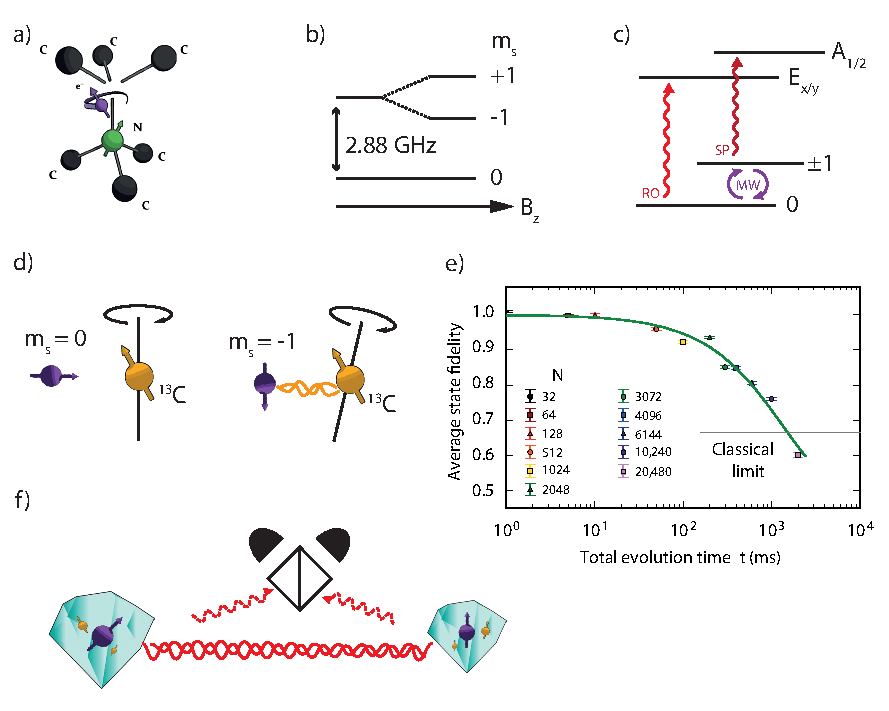
\includegraphics[width=\textwidth]{images/figure1}
	\caption{The \ac{NV} centre as a quantum network node. 
		a) The \ac{NV} is an atomic defect in diamond consisting of a neighbouring substitutional nitrogen atom and a vacancy.
		b) After capturing an electron from the environment the centre becomes negatively charged (\ac{NV}${}^-$) and forms a ground state spin triplet with a zero field splitting of \SI{2.88}{GHz}. An external magnetic field $B_z$ lifts the $m_s = \pm 1$ degeneracy \cite{Doherty2013}.
		c) At cryogenic temperatures (\SI{4}{K}) spin selective optical transitions allow high fidelity single-shot readout (\textsc{RO}) and initialization via spin pumping (\textsc{SP}) \cite{Robledo2011}. Microwave (\acs{MW}) pulses allow coherent manipulation of the spin state.
		d) Non-purified diamond presents a \SI{1.1}{\percent} natural abundance of ${}^{13} C$ atoms ($S = 1/2$) which couple to the \ac{NV} centre via a distance-dependent hyperfine coupling. This enables selective addressing of these  ${}^{13} C$ atoms and universal gates have been shown, making them a good candidate to act as quantum memories \cite{Taminiau2014}.
		e) \acf{DD} sequences, tailored to the unique ${}^{13} C$ environment of each \ac{NV} centre, extend coherence times of the electronic spin from ${T_2}^* \approx $ \SI{5}{\micro s} to ${T_2}^{DD} > $ \SI{1}{s}. Adapted from Ref.~\cite{Abobeih2018}.
		f) The combination of these properties makes it possible to entangle remote \ac{NV} centres via photon mediated protocols and run complex schemes such as entanglement purification and loop-hole free tests of Bell inequalities \cite{Kalb2017, Hensen2015}.}
	\label{fig:nv_summary}
\end{figure}

Recent work from our group demonstrated the on-demand generation of remote entanglement between two \ac{NV} centres with rates up to \SI{39}{\Hz} \cite{Humphreys2018}. Such high rates, three orders of magnitude higher than previous results on the same platform, are a consequence of moving from a two-photon detection protocol, such as the one used in Ref.~\cite{Hensen2015}, to a single-photon protocol.

While two-photon protocols can produce very high fidelity states and are not sensitive to the optical phase difference of the interfering photons, they scale quadratically in photon losses. This restricted entanglement generation with such protocols on the \ac{NV} platform to the \SI{}{mHz} regime. 
On the other hand, single photon protocols, although they require optical phase stability, scale linearly with photon losses. \autoref{fig:sce_scheme}a summarises the \ac{SCE} protocol used in Ref.~\cite{Humphreys2018}.

\begin{figure}[h]
%	\missingfigure[figwidth=\textwidth, figheight=0.6\textwidth]{The SCE protocol. Also new vs. old comparison}
	\centering
	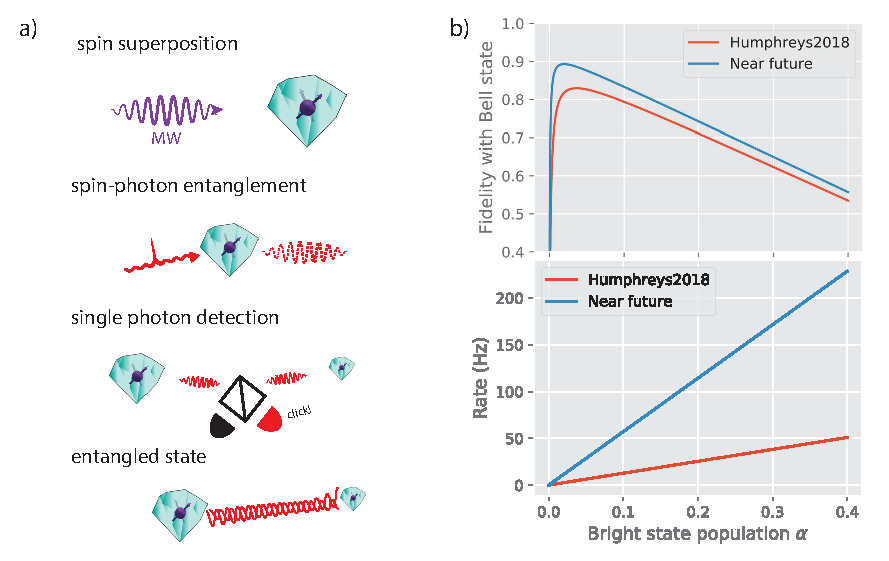
\includegraphics[width=0.9\textwidth]{images/figure2}
	\caption{The \acf{SCE} protocol.
	a) Two remote \acp{NV} are each put in a superposition state $\ket\alpha = \sqrt\alpha\ket\uparrow + \sqrt{1-\alpha}\ket\downarrow$ via a \ac{MW} pulse.
	A laser pulse resonant with the $\ket\uparrow$ state entangles the presence of a photon with the state of each \ac{NV}.
	The two photonic modes interfere on a \ac{BS}.
	The detection of a single photon heralds the entanglement between the \acp{NV}.
	b) Comparison of fidelity and rate of the \ac{SCE} protocol between Ref.~\cite{Humphreys2018} and near-future experiments (see \autoref{tab:sce_params}).}
	\label{fig:sce_scheme}
\end{figure}

\section{Genuine remote multipartite entanglement}
\label{sec:multipartite}
A two-particle state can either be entangled or separable. When three or more particles are involved in the state, there are more possibilities. The state can be fully separable, where each of the systems can be described independently of the others, partially separable, where some systems are entangled with each other but not all of them are, and genuinely entangled, where none of the systems are separable from each other.
It is possible to further categorise genuinely entangled states: if it is possible to transform one state into another via \ac{SLOCC}, then we say that the two states are \ac{SLOCC}-equivalent.

There are then two categories of triparite genuinely entangled states: the ones that are \ac{SLOCC}-equivalent to the \ac{GHZ} state, $\ket{\text{GHZ}} = (\ket{000} + \ket{111})/\sqrt 2 $, and the ones that can be transformed into the W state, $\ket{\text{W}} = (\ket{001} + \ket{010} + \ket{100})/\sqrt 3 $. While the W state has the interesting feature of maintaining entanglement even if some of the parties are lost, the \ac{GHZ} is usually considered more powerful and most quantum network protocols use a GHZ state as a resource \cite{Guehne2009}. 

\subsection{State generation}

Generation of remote GHZ states have been demonstrated on the photonic platform \cite{Bouwmeester1999}, and local GHZ states have been generated with \ac{NV} centres \cite{Neumann2008, vanDam2018}. Moving beyond two-node experiments requires the generation of remote genuine multipartite entanglement. \autoref{fig:3node_scheme} shows the proposed experimental gate circuit to generate a GHZ state among three remote \ac{NV} centres.

\begin{figure}[h]
%	\missingfigure[figwidth=\textwidth, figheight=0.6\textwidth]{The 3-node scheme. Experimental sequence, phase stabilisation.}
	\centering
	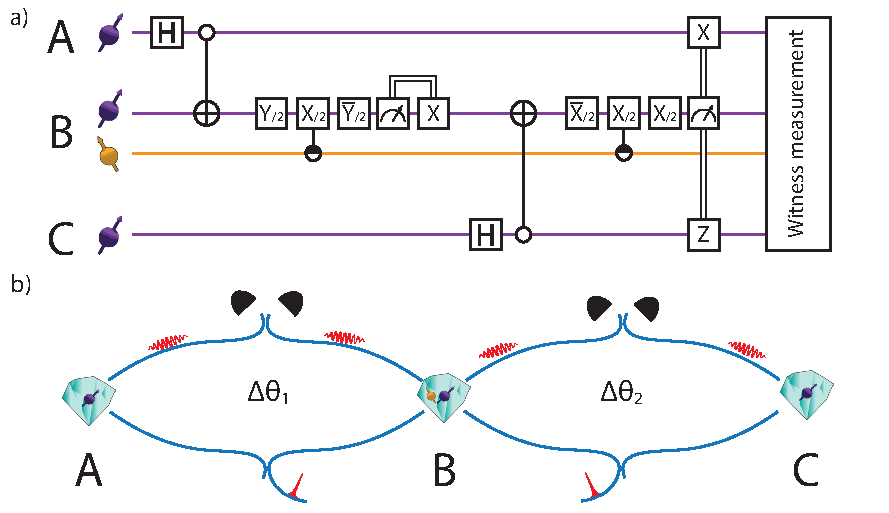
\includegraphics[width=\textwidth]{images/figure3}
	\caption{
		Generation of a remote GHZ state with three \ac{NV} centres.
		a) The experimental gate circuit: A first round of \acf{SCE} between nodes A and B. Subsequently node B performs a \textsc{SWAP} gate between the electronic spin and the carbon atom. Node B is then ready to run \ac{SCE} again, this time with node C. Finally a local controlled-operation on node B, followed by a measurement of the electron and announcement of the result creates the desired state. The entanglement witness can then be measured.
		b) Layout of the two interferometers to be used. The first one connects A with B, for the first round of \ac{SCE}, and the other interferometer connects B with C for the final round of \ac{SCE}. The two optical phases differences $\Delta\theta_1$ and $\Delta\theta_2$ need to be stabilised during the entanglement attempts. The physical implementation of the interferometer will make use of an optical switch, such that the same two detectors can be used for both rounds of \ac{SCE}.
	}
	\label{fig:3node_scheme}
\end{figure}

The experiment requires three experimental setups. Two of them, named LT3 and LT4 (Low-Temperature) are the same setups used in Refs.~\cite{Kalb2017, Humphreys2018}.
In the first year of my Ph.D. I built a new setup, named LT5, which has the same functionalities of the other setups and some upgrades to make it easier to use and increase the performance. The new setup is in a new laboratory, approximately \SI{20}{m} from the other two setups, which are \SI{1}{m} apart.

\begin{table}
	\begin{center}
		\begin{tabular}{lccccccc}
			\toprule
			& $p_\text{det}$ & $\sigma_\theta$ & $p_\text{2exc}$ & $\mathcal V$ & $N_{1/e}$ & $t_\text{ent}$ & $B_z$\\
			\hline
			Ref. \cite{Humphreys2018, Kalb2017} & \SI{3E-4}{} & \SI{14}{\degree} & 0.04 & 0.80 & 275 & \SI{5.5}{\micro s} & \SI{400}{G}\\ 
			\hline 
			Near-future & \SI{1E-3}{} & \SI{20}{\degree} & 0.02 & 0.90 & 1000 & \SI{3.5}{\micro s}&\SI{2000}{G}\\ 
			\bottomrule 
		\end{tabular}
	\end{center}
	\caption{Comparison of experimental parameters for \ac{SCE}. $p_\text{det}$ is the probability of detecting a photon in the \ac{ZPL}. $\sigma_\theta$ is the phase uncertainty of the stabilised interferometer. $p_\text{2exc}$ is the probability that the \ac{NV} had already been excited during the pulse if a photon is detected after the pulse. $\mathcal V$ is the visibility of the \ac{TPQI}. $N_{1/e}$ is the lifetime of the quantum memory (see main text). $t_\text{ent}$ is the duration of one entanglement attempt. $B_z$ is the external magnetic field applied to the \ac{NV}.}
	\label{tab:sce_params}
\end{table}

In \autoref{fig:sce_scheme}b there is a comparison between the results in Ref.~\cite{Humphreys2018} and estimated entanglement fidelities and rates with near-future experimental parameters (reported in~\autoref{tab:sce_params}). The increased detection efficiency, visibility and entanglement attempt speed will be a product of better classical control and optical components in the setups. The reduced probability of double excitation arises from an optimisation of the optical $\pi$ pulse shape and length. The phase uncertainty is estimated to be higher (i.e.~worse) due to the requirement of running the phase stabilisation faster and over longer distances. The increase in memory lifetime will be discussed in the next paragraphs.
 
After the first round of \ac{SCE} is executed, the state of the central node needs to be saved on a memory qubit. This will be done via a SWAP operation similar to the one used in Ref.~\cite{Kalb2017}.
A second round of \ac{SCE} will then take place, which will have a timeout, because of the decoherence of the first entangled state. If a second \ac{SCE} is successful within the timeout window, a local controlled gate on the central node will entangle the electron and carbon, therefore generating a 4-qubit entangled state. By measuring the electron of the central node, and feeding back the result to the other nodes it is possible to generate a GHZ state among the three nodes.

It is essential, for the success of the protocol, to be able to preserve the first entangled state while the second is being generated. While the state of the electronic spin of node A will be preserved using \ac{DD} sequences, and can reach up to \SI{1}{s} of coherence time \cite{Abobeih2018}, the nuclear spin on node B will be affected by the attempts to generate entanglement on the electronic spin. The main cause of this decoherence are errors in the \ac{MW} pulses used in the entanglement generation sequence \cite{Kalb2018}. These errors have limited the \emph{lifetime}\footnote{Here \emph{lifetime} does not directly refer to a time, but rather to the number of entanglement attempts necessary to decrease the length of the Bloch vector to $1/e$ of the original value.} $N_{1/e}$ of the quantum memory to $\approx 275$ entanglement attempt in past works \cite{Kalb2017}. As proposed in Ref.~\cite{Kalb2018}, an avenue to increase the resilience of the quantum memory to the network activity is to increase the external magnetic field applied to the sample. This will make it possible to run the \ac{MW} pulses in the entanglement generation sequence at a higher rate, therefore reducing the effect of their errors on the quantum memory. We have updated one of the setups (LT3) to run with a higher magnetic field of \SI{2000}{G} (instead of \SI{400}{G}). This should directly improve $N_{1/e}$ to $\approx 1000$.

\subsection{State characterisation}

An efficient way to show that a state is entangled is measuring entanglement witnesses \cite{Guehne2009}. An entanglement witness is quantity that distinguishes  a specific entangled state from separable ones. For example the quantity $\mathcal W_\text{GHZ} = \mathbb{1}/2 - \ket{\text{GHZ}}\bra{\text{GHZ}}$ is negative on genuine multipartite states (up to a certain noise) and positive for all separable and biseparable states. Measuring a negative value for $\mathcal W_\text{GHZ}$ is therefore a witness of a genuine multipartite entangled state. In order to investigate the feasibility of generating such a state with our experimental setup we perform simulations based on near-future parameters (see \autoref{tab:sce_params}). There are two parameters that we can tweak during the experiments: 1) the timeout for the generation of the second entangled state and 2) the bright state population $\alpha$ for the second round of \ac{SCE}. Note that for the first round of \ac{SCE} $\alpha$ is chosen such that the state with the highest possible fidelity is generated. In \autoref{fig:witness} the expected value of $\mathcal W_\text{GHZ}$  is plotted while varying those two parameters. A negative value of the witness (i.e. a fidelity of the generated state with the GHZ state $\mathcal{F} > 1/2$) can be obtained with states generated in approximately one minute.

\begin{figure}
	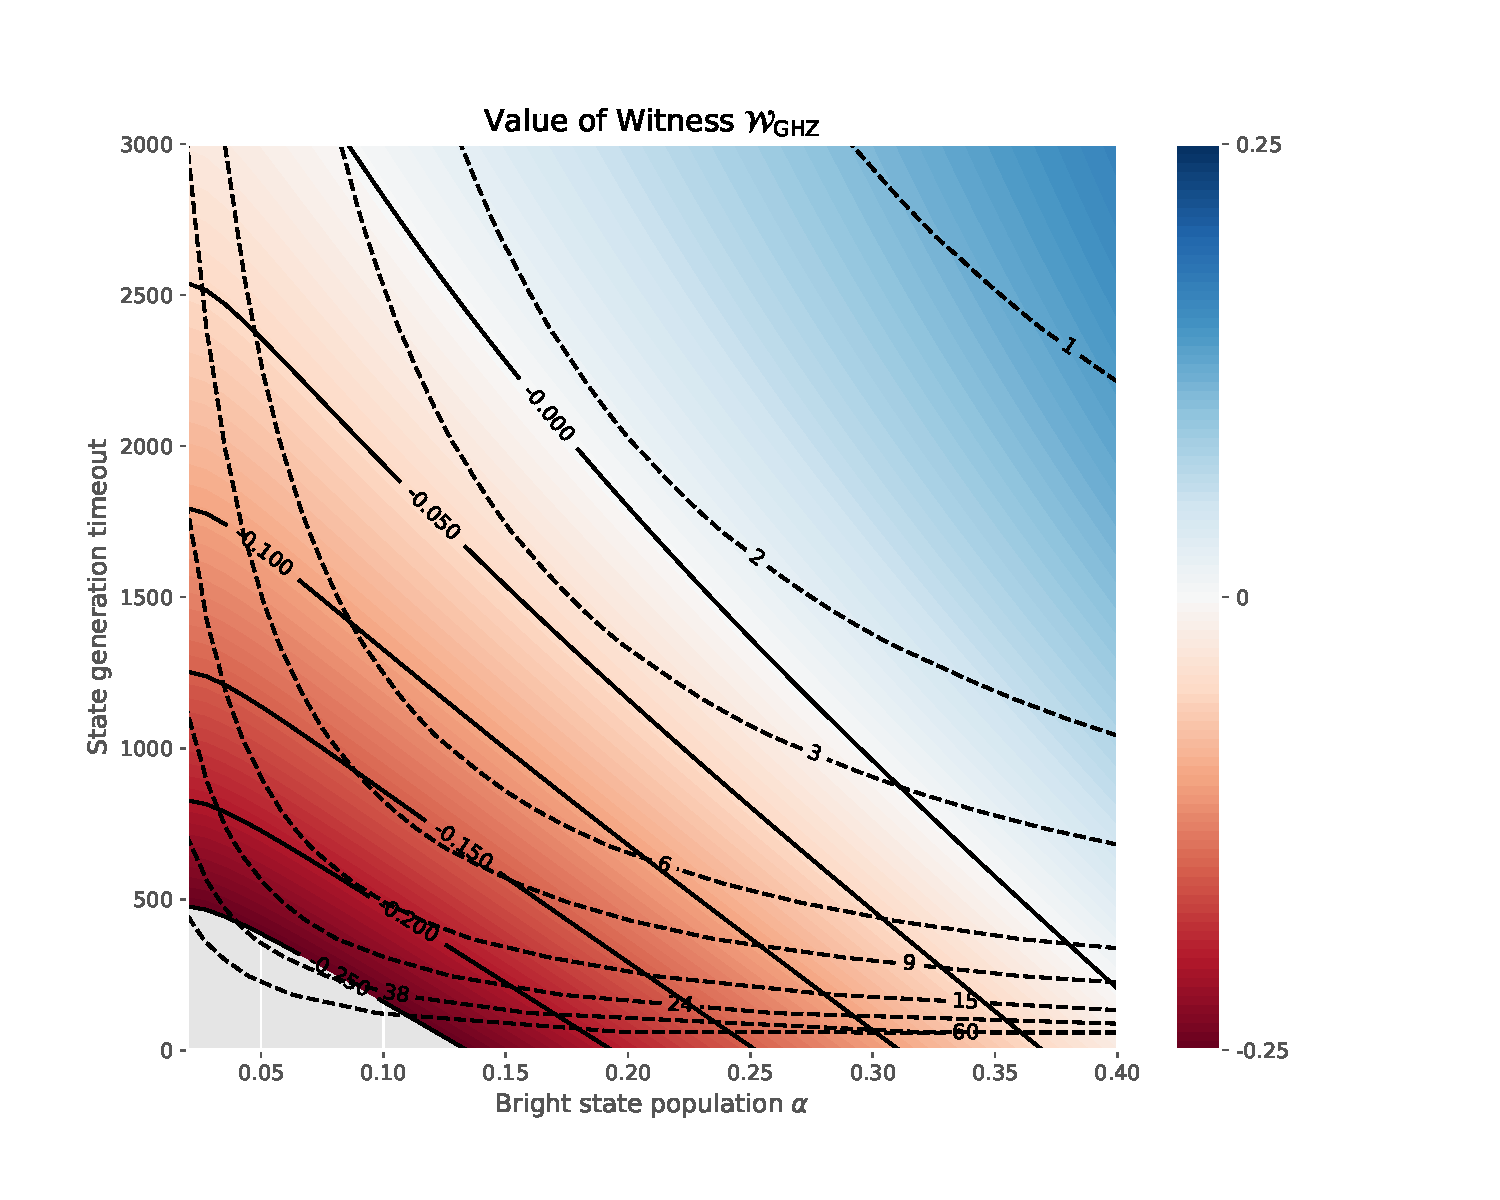
\includegraphics[width=\textwidth, trim=1cm 1cm 3cm 1cm 0cm]{../images/witness.pdf}
	\caption{Simulation of $\mathcal W_\text{GHZ}$ with near-future experimental parameters (see \autoref{tab:sce_params}). The solid lines on the plot represent curves where the witness value is constant. The dashed lines represent the time (in minutes) that it will take to generate such a state. The maximum achievable fidelity, in realistic experimental times, is therefore $\approx 0.75$.}
	\label{fig:witness}
\end{figure}

A Monte-Carlo simulation shows that, with near future experimental parameters (\autoref{tab:sce_params}), we would need $\approx 30$ hours of (non-consecutive) measurement to show that the witness is negative with a statistical significance of $3\sigma$, and $\approx 70$ hours for a $5\sigma$ significance.

\section{Link layer: a proof of concept}
\label{sec:link}

The Link layer is one of the layers of the network stack, a model that characterizes our current Internet without regard to the technological details of the various implementations, and makes it possible to build complex network applications in a device-agnostic manner. To build a Quantum Internet it is necessary to develop an analogous stack of layers.

The first layer of the stack is the Physical layer. This includes the quantum network nodes (in our case \ac{NV} centres) and the physical medium used to connect them (optical fibres). It also includes all the implementation specific instrumentation required to run the setups.

The Link layer is the next layer of the stack. In the Internet it takes care of reliably delivering data between adjacent nodes, without regard to the physical medium used by the nodes (cable, optical fibre, radio etc.).  In the Quantum Internet stack the Link layer will take care of reliably generating entanglement between two points directly connected, eventually through a quantum repeater.

The proposed experiment is a proof of principle of such a layer without the experimental complications that arise when the two nodes are far apart (thus requiring frequency conversion of the photons and/or a quantum repeater).
Our current multi-node experiments are controlled by a combination of time-deterministic micro-controllers and \acp{AWG}. The code and wave sequences used are highly experiment-specific, and need to be changed manually when a different experiment is required.

The objective of the experiment is to generate entanglement between two nodes using a prototype of the future Link layer.
An implementation-agnostic microcontroller with a custom operating system (nodeOS) would control each setup, sending commands to a second microcontroller that knows the specific of the system (in our case an \ac{NV} centre). A schematic of the experiment is depicted in \autoref{fig:link_layer_experiment}.

\begin{figure}
%	\missingfigure[figwidth=\textwidth, figheight=0.4\textwidth]{Link layer experiment scheme. The two NVs, the BS, the ADwins and the AWGs. On top of that the two nodeOS controller, talking to each other.}
	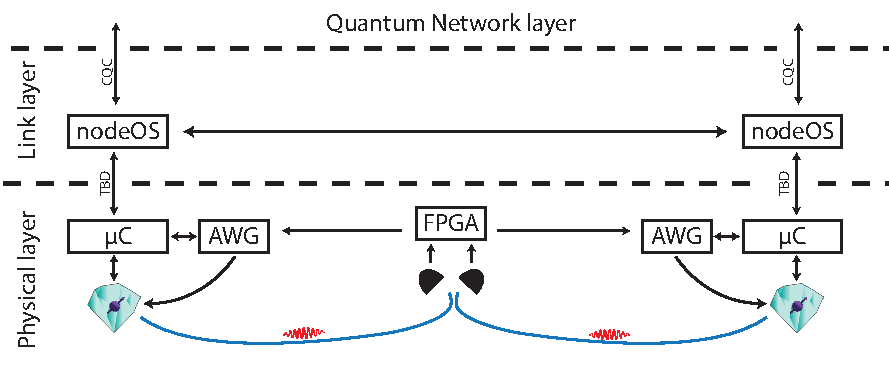
\includegraphics[width=\textwidth]{images/figure4}
	\caption{Link layer experimental scheme. 
		In the Physical layer two \ac{NV} centre nodes will be connected via an optical link (like in the \ac{SCE} protocol). Each node has a time-deterministic microcontroller ($\mu C$) that controls the node on a \SI{}{\micro s} time scale. Tasks that require \SI{}{\nano s} resolution are handled by an \acf{AWG}. At the detection point, a \acf{FPGA} heralds entanglement generation and communicate success (or failure) to the nodes.
		In the Link layer a microcontroller for each node will run a custom operating system (nodeOS) which is not aware of the experimental details of the Physical layer, and only knows some details of the  implementation to perform real time optimization of the resources. It will communicate with the experimental setup via a protocol currently being developed, the name of which is still to be decided (TBD). This will allow the Link layer to generate entanglement and to perform quantum gates without the need to reprogram the experimental setup. The nodes on the Link layer will communicate with each other via a classical link (for example Internet). In the future they will communicate with the layer above, the Quantum Network layer, via a protocol called \acf{CQC}, which is being developed at QuTech.
	}
	\label{fig:link_layer_experiment}
\end{figure}

The nodeOS controllers will communicate with each other using a direct classical link (an optical fibre, for example), while in the future implementations they would communicate on the Internet. The communication with the Physical link will use a protocol, currently in development, that will later be used on a metropolitan scale in the Demonstrator project.
The Link layer will also be able to execute simple quantum operations on the entangled qubits, making it possible to run different small-scale quantum programs without the need to reprogram the experimental setups.
The next layer of the stack will be the Quantum Network layer, which will communicate with the nodeOS on the Link layer with a protocol called \acf{CQC} (also in development).

\section{Entanglement teleportation}
\label{sec:teleportation}
Teleportation of states among the nodes of a quantum network is needed to successfully run quantum applications. Teleportation of single qubits has been shown on the \ac{NV} platform by our group \cite{Pfaff2014} and on several other platforms \cite{Takeda2013, Wang2015, Valivarthi2016}.
With four network nodes it is possible to deterministically teleport an entangled state to two nodes that are not directly connected, allowing them, for example, to run \ac{QKD}. \autoref{fig:ent_teleport} depicts the experimental scheme. 

\begin{figure}
%	\missingfigure[figwidth=\textwidth, figheight=0.4\textwidth]{Entanglement teleportation experimental scheme.}
	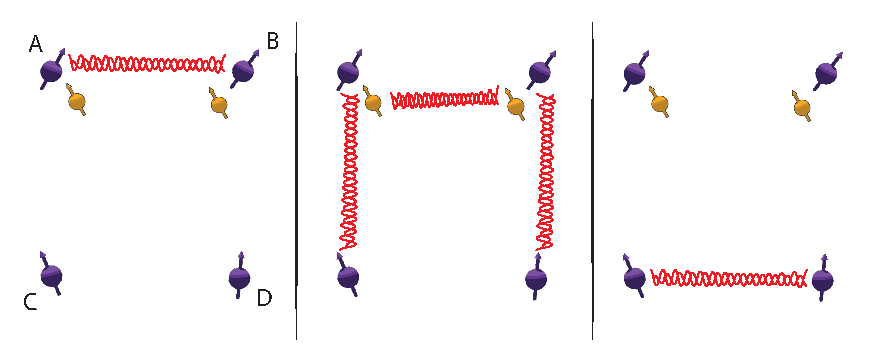
\includegraphics[width=\textwidth]{images/figure5}
	\caption{Entanglement teleportation experimental scheme. Nodes A and B generate an entangled state with the \ac{SCE} protocol. The state is swapped to the respective memories. A generates entanglement with C, while B generates entanglement with D. A and B perform a joint state measurement and announce their results. C and D share an entangled state. }
	\label{fig:ent_teleport}
\end{figure}

A fourth \ac{NV} node will be built to perform this experiment, and two of the four nodes (A and B) will require a ${}^{13}C$ quantum memory. The same near-future experimental parameters described in \autoref{sec:multipartite} will also allow this experiment to be performed. In particular, the lifetime $N_{1/e}$ of the quantum memories will play an important role: if the lifetime becomes comparable to the required number of entanglement attempts, the protocol could be executed on-demand. 

\section{Client-Server secure delegation}
\label{sec:delegation}

One of the key features of quantum networks is \ac{BQC}. A client, without any quantum computation power but the ability to generate single qubit states, interacts with an untrusted quantum server, capable (or not) of universal quantum computation. Quantum mechanics allows for a protocol where the server will execute for the client a computation, without being able to access the client's information, computation or results. The classical analogue is based on the assumption of the server's (or adversary's) limited computational power (just like RSA encryption).

A proof of principle experiment on the photonic platform was realized in 2012 \cite{Barz2012}. The proposed experiment on the \ac{NV} platform would follow the same experimental scheme, while allowing for an heralded execution.

The client would teleport, one at a time, random quantum states of the form $\ket\theta_j = (\ket 0 + e^{i \theta_j}\ket 1)/\sqrt 2$, with $\theta_j \in \lbrace0, \pi/4,\ldots,7\pi/4\rbrace$. The server, upon receiving the qubits, stores them in quantum memories and applies C-Phase gates to consecutive qubits.
At this point the client will communicate which measurements to perform (and in which bases). This allows the client to perform universal quantum computation, without sharing private information with the server. The readout bases, and the measurement outcomes, must be combined with the knowledge of the initial states (that only the client has) to obtain information about the computation performed and/or the result.

To perform this experiment on our platform we need to teleport multiple qubits from the client node to the memories of the server node. An increase in the lifetime on the memories is necessary (by at least an order of magnitude with respect to the current value) to be able to run more than one round of \ac{SCE} generation while preserving the state of a memory qubit. There are several options to increase the memory lifetime: a first possibility is to apply an even higher magnetic field (\SI{0.5}{T} or more), which would decrease the effect of \ac{MW} errors by making the pulses closer together (see Ref~\cite{Kalb2017}). A drawback of this approach is the need for vector sources that would need to reach up to \SI{20}{GHz}, and a new cryostat design that could house the needed magnet and deliver such high frequency signals with acceptable attenuation. A second option is to use \ac{RF} pulses to decouple the memory qubit from the environment, which would only require the additional mixing of \ac{RF} and \ac{MW} signals with respect to the current setup \cite{Bradley2018}. 
A third alternative, which is being researched in our group, is the combined use of close-by \ac{NV} centres. One of the \ac{NV} centres is used as an optical interface to generate remote entanglement. Once entanglement is established, the state can be swapped to the second \ac{NV} centre, which has then access to several quantum memories. In this way the memories would not experience the decoherence due to the entanglement generation attempts.

\section{Ph.D. time-line}
The Gantt Chart with the proposed Ph.D time-line is in \autoref{fig:phdtimeline}.
\begin{figure}[htb!]
	\begin{center}
		\begin{ganttchart}[
			hgrid,
			vgrid,
			expand chart=\textwidth
			]{1}{12}
			\gantttitle{Year 2}{4} \gantttitle{Year 3}{4} \gantttitle{Year 4}{4}\\
			\ganttbar{3-Node entanglement}{1}{2} \ganttnewline
			\ganttbar{Link layer demonstration}{3}{5} \ganttnewline
			\ganttbar[
			bar/.append style={fill=black!10,pattern=north east lines}
			]{Build $4^\text{th}$ setup}{4}{5} \ganttnewline
			\ganttbar{Entanglement teleportation}{6}{8} \ganttnewline
			\ganttbar{Secure delegation}{9}{10} \ganttnewline
			\ganttbar{Thesis writing}{11}{12}
		\end{ganttchart}
	\end{center}
	\caption{Proposed Ph.D. time-line: \emph{3-Node entanglement} is discussed in \autoref{sec:multipartite}. \emph{Link layer demonstration} in \autoref{sec:link}. \emph{Build $4^\text{th}$ setup} will not be a full time activity, but rather support to another Ph.D. student. \emph{Entanglement teleportation} is discussed in \autoref{sec:teleportation}, and \emph{Secure delegation} in \autoref{sec:delegation}. The last six months will be used to write the Thesis.}
	\label{fig:phdtimeline}
\end{figure}

\section{Graduate school progress}
\subsection{Courses}
I attended (or I am currently attending) the following courses:
\begin{itemize}
	\item Collaboration across disciplines (2 GSC)
	\item PhD Start-up (2 GSC)
	\item Conversation skills (2 GSC)
	\item Casimir Spring School 2018 (1GSC)
	\item Casimir Course - Programming (5 GSC)
	\item Casimir Course - Electronics for Physicists (5 GSC)
	\item QuTech Academy - Quantum Communication and Cryptography (5 GSC)
\end{itemize}

\subsection{Supervision}
I have been supervising Hans K. C. Beukers, a MSc student, since February 2018. Hans has been working on setup improvements and techniques that, if successful, will increase the lifetime of our memory qubits. He will graduate in February 2019.

\subsection{Outreach}
As an \ac{ESR} in the \ac{MSCA} \ac{ITN} Spin-NANO, I have to carry out outreach activities regarding my research field to the wider audience. I have currently carried out two outreach activities:
\begin{itemize}
	\item January 2018, Sheffield, UK. Introduction to quantum- and nano-technologies to local high-school students, as part of an \ac{ITN} meeting.
	\item September 2018, Brussels, BE. Two days stand about quantum technologies at the European Researchers Night, EU Parlamentarium, mainly to children between 5 and 10.
\end{itemize}

\section*{Acknowledgements}
\addcontentsline{toc}{section}{Acknowledgements}
I would like to thank Sophie Hermans, Simon Baier, Hans Beukers, Bas Drikse and Axel Dahlberg for helpful discussions on the future experiments.

%\section*{Appendix}
%\addcontentsline{toc}{section}{Appendix}
%\renewcommand{\thefigure}{A\arabic{figure}}
%\setcounter{figure}{0}
%
%\begin{figure}[h!]
%	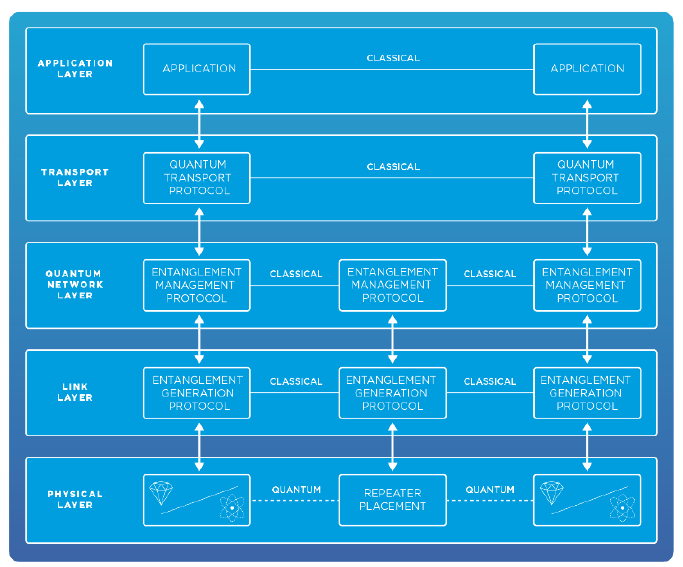
\includegraphics[width=\textwidth]{images/network_stack.png}
%	\caption{Proposed Quantum Internet stack\todo[inline]{Some description here? Can I even put it here? Need to cite the proposal. }}
%	\label{fig:network_stack}
%\end{figure}

\printbibliography[heading=bibintoc]
\end{document}          
